%!TEX root=thesis.tex

\chapter{Methods} % Reinforcement Learning for Hamiltonian Engineering

% TODO make sure it's clear what the goal is: Hamiltonian engineering

% physical constraints
% parameters for sequences

This section describes the simulation methods and RL algorithm used in this work. The implementation of both can be found at \url{https://github.com/wjkaufman/rl_pulse}.

\section{Simulated Spin Systems}

Isolated spin systems composed of a small number of spins can be easily simulated on a classical computer. Because the Hilbert space grows exponentially as the spins increase ($2^N$ basis states for $N$ spins and $2^{2N}$ matrix elements for operators), it quickly becomes impractical to simulate large numbers of spins. To balance the need to capture dipole interactions and to decrease simulation time, $N=3$ spin-1/2 systems were used in the reinforcement learning algorithm, and $N=4$ spin-1/2 systems were used to evaluate pulse sequences. The QuTiP Python package was used for all simulations \cite{Johansson_2013}.

In any real physical system, system-environment interactions are present and the spin system must be treated as open, but for simulation purposes the system is assumed to be isolated.
Consequently, the dynamics are given by unitary time-evolution operators. In principle, though, simulations of open quantum systems could be used with reinforcement learning algorithms, and may in fact lead to better control by accounting for non-unitary system dynamics.

For each simulated $N$-spin system, the chemical shift strengths $\{\delta_j\}_j$ and the dipolar coupling strengths $\{d_{jk}\}_{j,k}$ are drawn from normal distributions
\begin{align*}
    \delta_j &\sim \mathcal{N}(\mu=0, \sigma=1) \\
    d_{jk} &\sim \mathcal{N}(\mu=0, \sigma=D)
\end{align*}
so that the energy scale of the system is defined by the standard deviation of the chemical shifts. The parameter $D$ controls the regime of the spin system, where $D \gg 1$ is a ``strongly coupled'' spin system and $D \ll 1$ is ``weakly coupled.'' We focus on strongly coupled spin systems, and set $D = 100$ unless otherwise specified. With the chemical shift and dipolar coupling strengths, the internal Hamiltonian $H_{\text{int}}$ can be calculated (see equation~\ref{eq:nmr-ham}).

% As an example, in a $3$-spin system, there will be three chemical shift terms, six dipolar coupling terms, and $H_{\text{int}}$ will be an $8
% \times 8$ Hermitian matrix.

Once $H_{\text{int}}$ has been calculated, the free evolution propagator $U(\tau) \defeq U_\tau$ can be calculated via matrix exponentiation (see equation~\ref{eq:propagator-ti})
and
the pulse operators $\{ U_X, U_{\overline{X}}, U_Y, U_{\overline{Y}} \}$ can be calculated using equation~\ref{eq:X-pulse}.

Because the (random) choices of chemical shift and dipolar coupling strengths affect the dynamics of the spin system, an ensemble of spin systems was used both in the reinforcement learning algorithm and in evaluation of pulse sequences.
Each spin system used different random chemical shift and dipolar coupling strengths drawn from the same distributions (i.e. the dipolar strength parameter $D$ was the same for all systems). If experimental imperfections were also included, then each system also used different random errors.
It was found that using ensembles of 50 spin systems reduced the variance in fidelity enough while keeping runtimes relatively short, so
the reinforcement learning algorithm used 50 spin systems and evaluation used 100 spin systems.

To assess the performance of a pulse sequence for a Hamiltonian engineering problem, the pulse sequence propagator is compared to the target propagator given by
\[
U_{\text{target}} = \exp\left\{ -i H_{\text{eff}} T \right\}
\]
Under ideal conditions, the two propagators should be ``close'' in some way. One measure of ``closeness'' is the following fidelity function for two unitary operators
\begin{equation}
    \text{fidelity}(U, U_\text{target}) = \left| \frac{\Tr{
        U^\dagger U_\text{target}
    }}{\Tr{\identity}} \right|
\end{equation}
The fidelity approaches $1$ as the unitaries get ``closer'' and the average Hamiltonian approaches the target Hamiltonian, and approaches $0$ as the unitaries get further apart.

\section{Reinforcement Learning Implementation}\label{sec:methods-RL}

As explained previously,
the reinforcement learning methodology is sufficiently general to be applied to a wide range of problems in a variety of different ways.  The specific application of RL to the Hamiltonian engineering problem is described below.

\subsection{Action Space and Representation}

In an NMR spectrometer, the actions we can perform, or the ``knobs'' we can turn, are the rf field amplitudes in equation~\ref{eq:nmr-ham-rf}.
% TODO change this reference to something in the rotating frame
% with two control amplitudes, makes much more sense
The spectrometer's electronics limit the strength and the granularity of the rf field,
but this still allows for a staggeringly large \emph{continuous} action space. Instead of allowing for continuous control of the rf field%
\footnote{
Which is precisely the action space used in gradient ascent pulse engineering (GRAPE) algorithms \cite{Khaneja-2005}, although it does not use RL.
}%
, we only consider a finite set of pulses, each with an interval of free evolution after the pulse. The set of pulses we use is the set of $\pi/2$ rotations about the x- or y-axis along with a ``null pulse'' or delay. The action set is represented as $\{ D, X, \overline{X}, Y, \overline{Y} \}$.



In the physical system, the actions correspond to unitary operators that determine the overall propagator. If the free evolution interval has length $\tau$, then the $D$ action corresponds to propagator
\[
D \longrightarrow U_{\tau} = \exp\{ -i H_{\text{int}} \tau \}
\]
And the other pulse actions have corresponding propagators
\begin{align*}
    X &\longrightarrow U_{\tau} U_X \\
    \overline{X} &\longrightarrow U_{\tau} U_{\overline{X}} \\
    Y & \longrightarrow U_{\tau} U_Y \\
    \overline{Y} &\longrightarrow U_{\tau} U_{\overline{Y}}
\end{align*}
Where $U_X$ is defined in equation~\ref{eq:X-pulse}. In the simulations, $\tau = 10^{-4}$ and the pulse width $t_p = 10^{-5}$ unless otherwise specified.
% TODO give any more justification to this?
% TODO mention Clifford gates/group?
See figure~\ref{fig:actions} for the relationship between rf field amplitudes, unitary operators, and the actions.

\begin{figure}[H]
    \centering
    % \scalebox{.8}{
    

\tikzset{every picture/.style={line width=0.75pt}} %set default line width to 0.75pt        

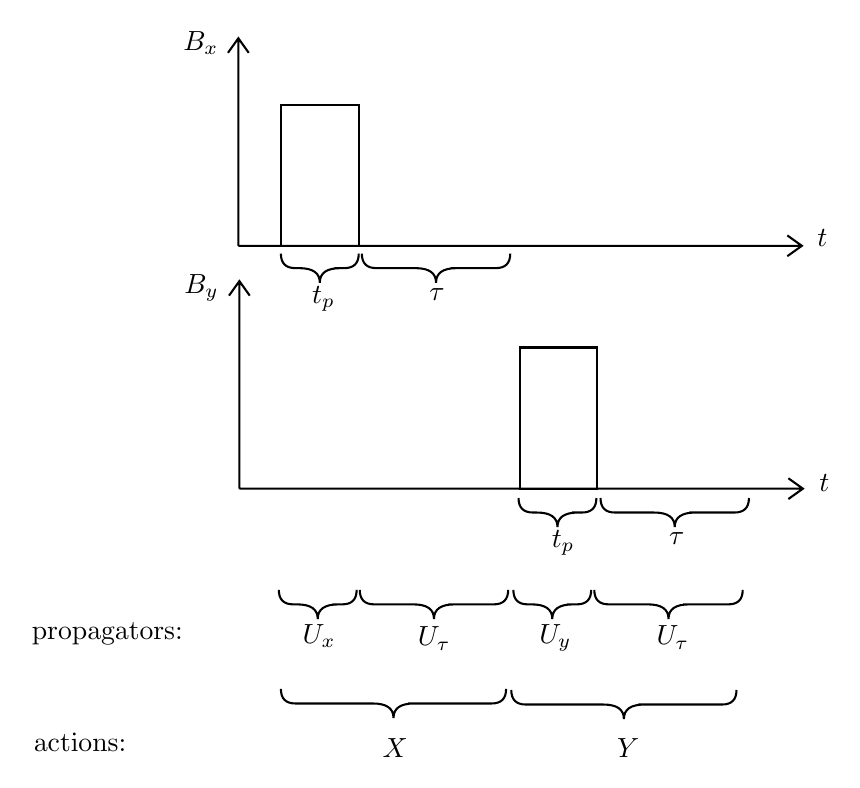
\begin{tikzpicture}[x=0.75pt,y=0.75pt,yscale=-1,xscale=1]
%uncomment if require: \path (0,416); %set diagram left start at 0, and has height of 416

%Shape: Axis 2D [id:dp22791562246140984] 
\draw  (114.5,118) -- (386,118)(114.5,18) -- (114.5,118) -- cycle (379,113) -- (386,118) -- (379,123) (109.5,25) -- (114.5,18) -- (119.5,25)  ;
%Shape: Axis 2D [id:dp9164432492680309] 
\draw  (115,235) -- (386.5,235)(115,135) -- (115,235) -- cycle (379.5,230) -- (386.5,235) -- (379.5,240) (110,142) -- (115,135) -- (120,142)  ;
%Shape: Rectangle [id:dp7980956907719897] 
\draw   (135,50) -- (172.5,50) -- (172.5,118) -- (135,118) -- cycle ;
%Shape: Rectangle [id:dp15473449548291585] 
\draw   (250,167) -- (287.5,167) -- (287.5,235) -- (250,235) -- cycle ;
%Shape: Brace [id:dp1991448415165501] 
\draw   (135,121.75) .. controls (135,126.42) and (137.33,128.75) .. (142,128.75) -- (143.75,128.75) .. controls (150.42,128.75) and (153.75,131.08) .. (153.75,135.75) .. controls (153.75,131.08) and (157.08,128.75) .. (163.75,128.75)(160.75,128.75) -- (165.5,128.75) .. controls (170.17,128.75) and (172.5,126.42) .. (172.5,121.75) ;
%Shape: Brace [id:dp9861614828174649] 
\draw   (249.5,239.5) .. controls (249.5,244.17) and (251.83,246.5) .. (256.5,246.5) -- (258.25,246.5) .. controls (264.92,246.5) and (268.25,248.83) .. (268.25,253.5) .. controls (268.25,248.83) and (271.58,246.5) .. (278.25,246.5)(275.25,246.5) -- (280,246.5) .. controls (284.67,246.5) and (287,244.17) .. (287,239.5) ;
%Shape: Brace [id:dp40037870153963473] 
\draw   (174,121.75) .. controls (174,126.42) and (176.33,128.75) .. (181,128.75) -- (199.75,128.75) .. controls (206.42,128.75) and (209.75,131.08) .. (209.75,135.75) .. controls (209.75,131.08) and (213.08,128.75) .. (219.75,128.75)(216.75,128.75) -- (238.5,128.75) .. controls (243.17,128.75) and (245.5,126.42) .. (245.5,121.75) ;
%Shape: Brace [id:dp46052279120608] 
\draw   (289,239.5) .. controls (289,244.17) and (291.33,246.5) .. (296,246.5) -- (314.75,246.5) .. controls (321.42,246.5) and (324.75,248.83) .. (324.75,253.5) .. controls (324.75,248.83) and (328.08,246.5) .. (334.75,246.5)(331.75,246.5) -- (353.5,246.5) .. controls (358.17,246.5) and (360.5,244.17) .. (360.5,239.5) ;
%Shape: Brace [id:dp8265278999467868] 
\draw   (135,331.5) .. controls (135,336.17) and (137.33,338.5) .. (142,338.5) -- (179.25,338.5) .. controls (185.92,338.5) and (189.25,340.83) .. (189.25,345.5) .. controls (189.25,340.83) and (192.58,338.5) .. (199.25,338.5)(196.25,338.5) -- (236.5,338.5) .. controls (241.17,338.5) and (243.5,336.17) .. (243.5,331.5) ;
%Shape: Brace [id:dp6026156031175705] 
\draw   (246,332) .. controls (246,336.67) and (248.33,339) .. (253,339) -- (290.25,339) .. controls (296.92,339) and (300.25,341.33) .. (300.25,346) .. controls (300.25,341.33) and (303.58,339) .. (310.25,339)(307.25,339) -- (347.5,339) .. controls (352.17,339) and (354.5,336.67) .. (354.5,332) ;
%Shape: Brace [id:dp7151581075598589] 
\draw   (134,283.75) .. controls (134,288.42) and (136.33,290.75) .. (141,290.75) -- (142.75,290.75) .. controls (149.42,290.75) and (152.75,293.08) .. (152.75,297.75) .. controls (152.75,293.08) and (156.08,290.75) .. (162.75,290.75)(159.75,290.75) -- (164.5,290.75) .. controls (169.17,290.75) and (171.5,288.42) .. (171.5,283.75) ;
%Shape: Brace [id:dp09735422637765234] 
\draw   (173,283.75) .. controls (173,288.42) and (175.33,290.75) .. (180,290.75) -- (198.75,290.75) .. controls (205.42,290.75) and (208.75,293.08) .. (208.75,297.75) .. controls (208.75,293.08) and (212.08,290.75) .. (218.75,290.75)(215.75,290.75) -- (237.5,290.75) .. controls (242.17,290.75) and (244.5,288.42) .. (244.5,283.75) ;
%Shape: Brace [id:dp48107626773199663] 
\draw   (247,283.75) .. controls (247,288.42) and (249.33,290.75) .. (254,290.75) -- (255.75,290.75) .. controls (262.42,290.75) and (265.75,293.08) .. (265.75,297.75) .. controls (265.75,293.08) and (269.08,290.75) .. (275.75,290.75)(272.75,290.75) -- (277.5,290.75) .. controls (282.17,290.75) and (284.5,288.42) .. (284.5,283.75) ;
%Shape: Brace [id:dp02583834690299247] 
\draw   (286,283.75) .. controls (286,288.42) and (288.33,290.75) .. (293,290.75) -- (311.75,290.75) .. controls (318.42,290.75) and (321.75,293.08) .. (321.75,297.75) .. controls (321.75,293.08) and (325.08,290.75) .. (331.75,290.75)(328.75,290.75) -- (350.5,290.75) .. controls (355.17,290.75) and (357.5,288.42) .. (357.5,283.75) ;

% Text Node
\draw (86.5,13.4) node [anchor=north west][inner sep=0.75pt]    {$B_{x}$};
% Text Node
\draw (87,130.4) node [anchor=north west][inner sep=0.75pt]    {$B_{y}$};
% Text Node
\draw (148.5,136.15) node [anchor=north west][inner sep=0.75pt]    {$t_{p}$};
% Text Node
\draw (205,137.15) node [anchor=north west][inner sep=0.75pt]    {$\tau $};
% Text Node
\draw (264,253.65) node [anchor=north west][inner sep=0.75pt]    {$t_{p}$};
% Text Node
\draw (320.5,254.65) node [anchor=north west][inner sep=0.75pt]    {$\tau $};
% Text Node
\draw (182.5,353.9) node [anchor=north west][inner sep=0.75pt]    {$X$};
% Text Node
\draw (295.5,353.9) node [anchor=north west][inner sep=0.75pt]    {$Y$};
% Text Node
\draw (144,299.15) node [anchor=north west][inner sep=0.75pt]    {$U_{x}$};
% Text Node
\draw (199.5,300.15) node [anchor=north west][inner sep=0.75pt]    {$U_{\tau }$};
% Text Node
\draw (258,299.15) node [anchor=north west][inner sep=0.75pt]    {$U_{y}$};
% Text Node
\draw (314.5,299.65) node [anchor=north west][inner sep=0.75pt]    {$U_{\tau }$};
% Text Node
\draw (13.5,298) node [anchor=north west][inner sep=0.75pt]   [align=left] {propagators:};
% Text Node
\draw (14.5,351) node [anchor=north west][inner sep=0.75pt]   [align=left] {actions:};
% Text Node
\draw (392,108.4) node [anchor=north west][inner sep=0.75pt]    {$t$};
% Text Node
\draw (393,226.9) node [anchor=north west][inner sep=0.75pt]    {$t$};


\end{tikzpicture}

    % }
    \caption{The rf field amplitudes, the unitary operators, and corresponding actions.}
    \label{fig:actions}
\end{figure}

In principle, the actions could also be defined as pulses without a $\tau$ delay of free evolution and a delay action. However, in practice this leads to worse performance: for episodes with a fixed number of timesteps, the actions taken influence how much time elapses in the pulse sequence. As a result, the ``optimal'' performance is found to minimize the elapsed time by applying alternating pulses (e.g. $X, \overline{X}, X, \overline{X}, \dots$).
The unitary operator fidelity generally improves as the time interval decreases, so this is an unhelpful solution when pursuing high fidelity at longer time intervals.

\subsection{State Space and Representation}

The ``state'' can refer to the physics notion of state--such as the the density operator $\rho$ of a quantum system--or the RL notion of state--a particular context in which the agent must choose an action. They are closely related but not the same.
The ``physical'' state space is comprised of every reachable state $\rho(t)$ of the spin system given an initial thermalized state, the free evolution dynamics from $H_{\text{int}}$, and the control Hamiltonian given by the rf field $H_{\text{rf}}$.
In an RL context, however, the agent does not observe the complete state of the system at each point in time. Instead, the agent only knows the sequence of actions that have been performed on the system and any measurements that have been made on the system.
Therefore, a more representative state space for the RL problem is all possible sequences of actions performed on the system.%
\footnote{
Making measurements on the system could also be considered an action (measurement affects the physical state), and the resulting measurement outcome could be included in the state \cite{porotti2019coherent}. This possibility, however, is not explored here.
}
This is more ``realistic'' in the sense that the agent only knows what the experimenter would know, without getting any additional information ``for free.''
%This also simplifies the state representation with ensembles of spin systems.
% TODO what did I mean by this^???

\subsection{Reward Function}

% The fidelity approaches $1$ as the unitaries get ``closer'' and the average Hamiltonian approaches the target Hamiltonian, and approaches $0$ as the unitaries get further apart.
As mentioned above, the fidelity function takes on values between $0$ and $1$, where values close to $1$ are desirable.
However, a tenfold improvement in performance doesn't correspond to a tenfold increase in fidelity (take for instance a fidelity of 0.9 compared to 0.99). A suitable reward function is then calculated by
\begin{equation}
    r = -\log(1-\text{fidelity}(U_\text{actual}, U_\text{target}) + \epsilon)
\end{equation}
where $\epsilon>0$ ensures the reward isn't infinite.

\subsection{AlphaZero Algorithm}

As mentioned in the introduction, the AlphaZero algorithm has two main components: self-play and neural network training. The original publication and its supplementary materials has a complete description of the algorithm \cite{Silver1140}, but pseudocode is presented below as well.

During self-play, the agent iteratively constructs a pulse sequence by performing Monte Carlo Tree Search (MCTS) from the current state. From state $s_i$ (which is represented by the sequence of actions performed so far, $s_i = (a_0, \dots, a_i)$), the agent stochastically samples actions based on the prior probability from the policy $\pi$, the number of times the agent has already ``visited'' that action, and the average estimated reward (or value) of that branch of the tree. The agent is more likely to select actions that have a higher prior probability, a lower visit count, and a higher average reward. The exact formula for selection is given in algorithm~\ref{al:mcts},
and is a variant of the PUCT algorithm from \cite{Rosin:2011uu}.

The agent performs many rollouts of selecting actions, estimating the rewards, and updating visit counts and reward estimates along the particular sequence of actions. After a certain number of rollouts, the agent finally picks a particular action to perform by sampling from the empirical distribution of visit counts.
See figure~\ref{fig:mcts} for a visual depiction of the MCTS process.


{\setstretch{1.0}
\begin{algorithm}[H]
\KwData{Current state $s = (a_0, \dots, a_{i-1})$, policy and value networks $(\pi, v)$, number of rollouts $n_\text{roll}$, Dirichlet noise parameter $\alpha$, noise weight $w \in [0,1]$, PUCT parameters $c_\text{base}, c_\text{init}$}
\KwResult{Probabilities $\{p_k\}_k$ of selecting action $a_k$ from state $s$, and randomly sampled action $a$}
\BlankLine
Initialize root node associated with current state $s$ \;
Create child nodes of the root node corresponding to each action in the action space \;
Initialize set of statistics $\{ N(s,a_k)=0, W(s,a_k)=0, Q(s,a_k)=0, P(s,a_k)= \pi(s, a_k) \}_k$ for each child node $a_k$, where $N$ is the visit count, $W$ is the total value, $Q$ is the mean value, and $P$ is the prior probability from the policy network $\pi$ \;

Sample multivariate Dirichlet noise from $\text{Dir}(\alpha)$ and add it to the priors $\{P(s, a_k)\}_k$ \;
\For{$n_\text{roll}$ tree rollouts}{
Set $s_0 \leftarrow s$, $i \leftarrow 0$ \;
\While{$s_i$ is not a leaf node}{
Select a child node of $s_i$ associated with action $a_k$ by maximizing $Q(s_i, a_k) + U(s_i, a_k)$ where
\[
U(s, a) = C(s) P(s,a) \sqrt{N(s)}/(1+N(s,a))
\]
And $C(s) = \log((1+N(s) + c_\text{base})/c_\text{base}) + c_\text{init}$ \;
Let $s_{i+1} \leftarrow s_i + (a_k)$ and $i \leftarrow i + 1$ \;
}

\If{
the leaf node $s_L$ represents a pulse sequence with the desired length
}{
Calculate the fidelity of the pulse sequence in spin system ensemble \;
Calculate the reward $r$ from fidelity \;
}
\Else{
Evaluate the leaf node $s_L$ using $(\pi, v)$ to create child nodes of $s_L$ with initialized statistics $\{ N(s_L,a_k)=0, W(s_L,a_k)=0, Q(s_L,a_k)=0, P(s_L,a_k)= \pi(s_L, a_k) \}_k$, and an estimated reward $r = v(s_L)$ \;
}
For each of the nodes $s_i$ visited from $s_0$ to $s_L$, update the visit counts $N(s_i, a_i) = N(s_i, a_i) + 1$ and the values $W(s_i, a_i) = W(s_i, a_i) + r, Q(s_i, a_i) = \frac{W(s_i, a_i)}{N(s_i, a_i)}$ \;
}

Calculate the estimated probability $p_k \leftarrow N(s, a_k) / N(s)$ for each action $a_k$ \;
Randomly sample an action $a_k$ from the distribution $\{ p_k \}$ \;

\caption{Monte Carlo Tree Search (MCTS) for selecting the next action. \label{al:mcts}}
\end{algorithm}
}

\begin{figure}[H]
    \centering
    % \includegraphics[width=.7\textwidth]{MCTS.jpeg}
    % \scalebox{.8}{
    

\tikzset{every picture/.style={line width=0.75pt}} %set default line width to 0.75pt        

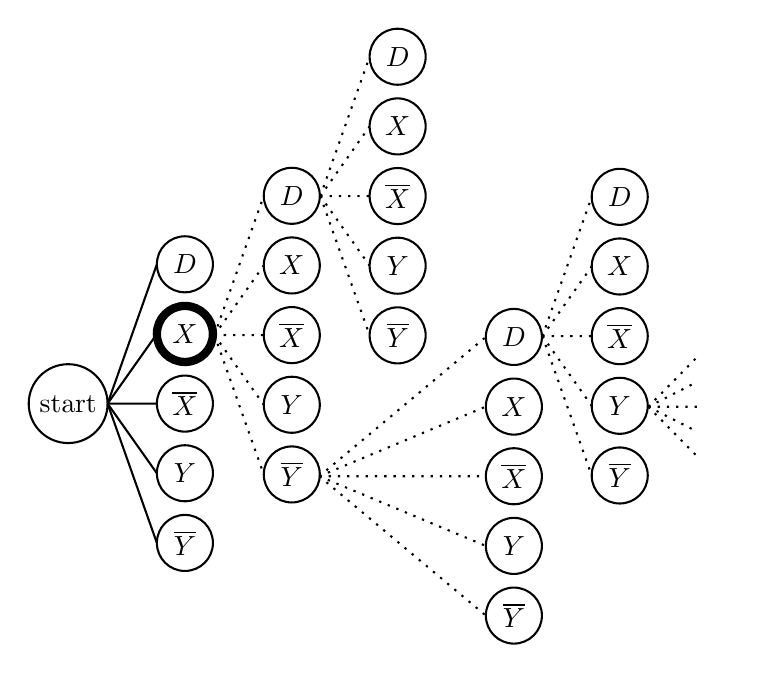
\begin{tikzpicture}[x=0.75pt,y=0.75pt,yscale=-1,xscale=1]
%uncomment if require: \path (0,383); %set diagram left start at 0, and has height of 383

%Straight Lines [id:da6767239887482572] 
\draw    (70.5,208.63) -- (94.25,175.06) ;
%Shape: Circle [id:dp6160154040167107] 
\draw   (32.5,208.63) .. controls (32.5,198.13) and (41.01,189.63) .. (51.5,189.63) .. controls (61.99,189.63) and (70.5,198.13) .. (70.5,208.63) .. controls (70.5,219.12) and (61.99,227.63) .. (51.5,227.63) .. controls (41.01,227.63) and (32.5,219.12) .. (32.5,208.63) -- cycle ;

%Shape: Circle [id:dp980766064746493] 
\draw   (94.25,141.5) .. controls (94.25,134.04) and (100.29,128) .. (107.75,128) .. controls (115.21,128) and (121.25,134.04) .. (121.25,141.5) .. controls (121.25,148.96) and (115.21,155) .. (107.75,155) .. controls (100.29,155) and (94.25,148.96) .. (94.25,141.5) -- cycle ;

%Shape: Circle [id:dp29813438855817054] 
\draw  [line width=3]  (94.25,175.06) .. controls (94.25,167.6) and (100.29,161.56) .. (107.75,161.56) .. controls (115.21,161.56) and (121.25,167.6) .. (121.25,175.06) .. controls (121.25,182.52) and (115.21,188.56) .. (107.75,188.56) .. controls (100.29,188.56) and (94.25,182.52) .. (94.25,175.06) -- cycle ;

%Shape: Circle [id:dp27671672588337426] 
\draw   (94.25,208.62) .. controls (94.25,201.16) and (100.29,195.12) .. (107.75,195.12) .. controls (115.21,195.12) and (121.25,201.16) .. (121.25,208.62) .. controls (121.25,216.08) and (115.21,222.12) .. (107.75,222.12) .. controls (100.29,222.12) and (94.25,216.08) .. (94.25,208.62) -- cycle ;

%Shape: Circle [id:dp11268971599796629] 
\draw   (94.25,275.75) .. controls (94.25,268.29) and (100.29,262.25) .. (107.75,262.25) .. controls (115.21,262.25) and (121.25,268.29) .. (121.25,275.75) .. controls (121.25,283.21) and (115.21,289.25) .. (107.75,289.25) .. controls (100.29,289.25) and (94.25,283.21) .. (94.25,275.75) -- cycle ;

%Shape: Circle [id:dp11266982300378847] 
\draw   (94.25,242.18) .. controls (94.25,234.72) and (100.29,228.68) .. (107.75,228.68) .. controls (115.21,228.68) and (121.25,234.72) .. (121.25,242.18) .. controls (121.25,249.64) and (115.21,255.68) .. (107.75,255.68) .. controls (100.29,255.68) and (94.25,249.64) .. (94.25,242.18) -- cycle ;

%Straight Lines [id:da0005946830674246062] 
\draw    (70.5,208.63) -- (94.25,208.62) ;
%Straight Lines [id:da7148795099260691] 
\draw    (70.5,208.63) -- (94.25,141.5) ;
%Straight Lines [id:da2783743734510492] 
\draw    (70.5,208.63) -- (94.25,242.18) ;
%Straight Lines [id:da1605478478685486] 
\draw    (70.5,208.63) -- (94.25,275.75) ;
%Straight Lines [id:da25097802387613777] 
\draw  [dash pattern={on 0.84pt off 2.51pt}]  (122,175.63) -- (145.75,142.06) ;
%Shape: Circle [id:dp337054674124885] 
\draw   (145.75,108.5) .. controls (145.75,101.04) and (151.79,95) .. (159.25,95) .. controls (166.71,95) and (172.75,101.04) .. (172.75,108.5) .. controls (172.75,115.96) and (166.71,122) .. (159.25,122) .. controls (151.79,122) and (145.75,115.96) .. (145.75,108.5) -- cycle ;

%Shape: Circle [id:dp6734169459600766] 
\draw  [line width=0.75]  (145.75,142.06) .. controls (145.75,134.6) and (151.79,128.56) .. (159.25,128.56) .. controls (166.71,128.56) and (172.75,134.6) .. (172.75,142.06) .. controls (172.75,149.52) and (166.71,155.56) .. (159.25,155.56) .. controls (151.79,155.56) and (145.75,149.52) .. (145.75,142.06) -- cycle ;

%Shape: Circle [id:dp22479699204389958] 
\draw   (145.75,175.62) .. controls (145.75,168.16) and (151.79,162.12) .. (159.25,162.12) .. controls (166.71,162.12) and (172.75,168.16) .. (172.75,175.62) .. controls (172.75,183.08) and (166.71,189.12) .. (159.25,189.12) .. controls (151.79,189.12) and (145.75,183.08) .. (145.75,175.62) -- cycle ;

%Shape: Circle [id:dp055836045919755994] 
\draw   (145.75,242.75) .. controls (145.75,235.29) and (151.79,229.25) .. (159.25,229.25) .. controls (166.71,229.25) and (172.75,235.29) .. (172.75,242.75) .. controls (172.75,250.21) and (166.71,256.25) .. (159.25,256.25) .. controls (151.79,256.25) and (145.75,250.21) .. (145.75,242.75) -- cycle ;

%Shape: Circle [id:dp7716751188113807] 
\draw   (145.75,209.18) .. controls (145.75,201.72) and (151.79,195.68) .. (159.25,195.68) .. controls (166.71,195.68) and (172.75,201.72) .. (172.75,209.18) .. controls (172.75,216.64) and (166.71,222.68) .. (159.25,222.68) .. controls (151.79,222.68) and (145.75,216.64) .. (145.75,209.18) -- cycle ;

%Straight Lines [id:da33500068657418713] 
\draw  [dash pattern={on 0.84pt off 2.51pt}]  (122,175.63) -- (145.75,175.62) ;
%Straight Lines [id:da6492159334152638] 
\draw  [dash pattern={on 0.84pt off 2.51pt}]  (122,175.63) -- (145.75,108.5) ;
%Straight Lines [id:da7484032093627121] 
\draw  [dash pattern={on 0.84pt off 2.51pt}]  (122,175.63) -- (145.75,209.18) ;
%Straight Lines [id:da11147051498905958] 
\draw  [dash pattern={on 0.84pt off 2.51pt}]  (122,175.63) -- (145.75,242.75) ;

%Straight Lines [id:da4324256339190172] 
\draw  [dash pattern={on 0.84pt off 2.51pt}]  (280,176.13) -- (303.75,142.56) ;
%Shape: Circle [id:dp3141653681630151] 
\draw   (303.75,109) .. controls (303.75,101.54) and (309.79,95.5) .. (317.25,95.5) .. controls (324.71,95.5) and (330.75,101.54) .. (330.75,109) .. controls (330.75,116.46) and (324.71,122.5) .. (317.25,122.5) .. controls (309.79,122.5) and (303.75,116.46) .. (303.75,109) -- cycle ;

%Shape: Circle [id:dp6862318414763178] 
\draw  [line width=0.75]  (303.75,142.56) .. controls (303.75,135.1) and (309.79,129.06) .. (317.25,129.06) .. controls (324.71,129.06) and (330.75,135.1) .. (330.75,142.56) .. controls (330.75,150.02) and (324.71,156.06) .. (317.25,156.06) .. controls (309.79,156.06) and (303.75,150.02) .. (303.75,142.56) -- cycle ;

%Shape: Circle [id:dp6298017846495424] 
\draw   (303.75,176.12) .. controls (303.75,168.66) and (309.79,162.62) .. (317.25,162.62) .. controls (324.71,162.62) and (330.75,168.66) .. (330.75,176.12) .. controls (330.75,183.58) and (324.71,189.62) .. (317.25,189.62) .. controls (309.79,189.62) and (303.75,183.58) .. (303.75,176.12) -- cycle ;

%Shape: Circle [id:dp841010081767361] 
\draw   (303.75,243.25) .. controls (303.75,235.79) and (309.79,229.75) .. (317.25,229.75) .. controls (324.71,229.75) and (330.75,235.79) .. (330.75,243.25) .. controls (330.75,250.71) and (324.71,256.75) .. (317.25,256.75) .. controls (309.79,256.75) and (303.75,250.71) .. (303.75,243.25) -- cycle ;

%Shape: Circle [id:dp24934148026454395] 
\draw   (303.75,209.68) .. controls (303.75,202.22) and (309.79,196.18) .. (317.25,196.18) .. controls (324.71,196.18) and (330.75,202.22) .. (330.75,209.68) .. controls (330.75,217.14) and (324.71,223.18) .. (317.25,223.18) .. controls (309.79,223.18) and (303.75,217.14) .. (303.75,209.68) -- cycle ;

%Straight Lines [id:da7454534180420143] 
\draw  [dash pattern={on 0.84pt off 2.51pt}]  (280,176.13) -- (303.75,176.12) ;
%Straight Lines [id:da5871561279842649] 
\draw  [dash pattern={on 0.84pt off 2.51pt}]  (280,176.13) -- (303.75,109) ;
%Straight Lines [id:da3506388826675355] 
\draw  [dash pattern={on 0.84pt off 2.51pt}]  (280,176.13) -- (303.75,209.68) ;
%Straight Lines [id:da3638734778566356] 
\draw  [dash pattern={on 0.84pt off 2.51pt}]  (280,176.13) -- (303.75,243.25) ;

%Straight Lines [id:da8858155616614573] 
\draw  [dash pattern={on 0.84pt off 2.51pt}]  (172.5,243.63) -- (252.75,210.06) ;
%Shape: Circle [id:dp007823309994931416] 
\draw   (252.75,176.5) .. controls (252.75,169.04) and (258.79,163) .. (266.25,163) .. controls (273.71,163) and (279.75,169.04) .. (279.75,176.5) .. controls (279.75,183.96) and (273.71,190) .. (266.25,190) .. controls (258.79,190) and (252.75,183.96) .. (252.75,176.5) -- cycle ;

%Shape: Circle [id:dp7127480050779221] 
\draw  [line width=0.75]  (252.75,210.06) .. controls (252.75,202.6) and (258.79,196.56) .. (266.25,196.56) .. controls (273.71,196.56) and (279.75,202.6) .. (279.75,210.06) .. controls (279.75,217.52) and (273.71,223.56) .. (266.25,223.56) .. controls (258.79,223.56) and (252.75,217.52) .. (252.75,210.06) -- cycle ;

%Shape: Circle [id:dp15768561663300074] 
\draw   (252.75,243.62) .. controls (252.75,236.16) and (258.79,230.12) .. (266.25,230.12) .. controls (273.71,230.12) and (279.75,236.16) .. (279.75,243.62) .. controls (279.75,251.08) and (273.71,257.12) .. (266.25,257.12) .. controls (258.79,257.12) and (252.75,251.08) .. (252.75,243.62) -- cycle ;

%Shape: Circle [id:dp6615602882865153] 
\draw   (252.75,310.75) .. controls (252.75,303.29) and (258.79,297.25) .. (266.25,297.25) .. controls (273.71,297.25) and (279.75,303.29) .. (279.75,310.75) .. controls (279.75,318.21) and (273.71,324.25) .. (266.25,324.25) .. controls (258.79,324.25) and (252.75,318.21) .. (252.75,310.75) -- cycle ;

%Shape: Circle [id:dp31467910906882635] 
\draw   (252.75,277.18) .. controls (252.75,269.72) and (258.79,263.68) .. (266.25,263.68) .. controls (273.71,263.68) and (279.75,269.72) .. (279.75,277.18) .. controls (279.75,284.64) and (273.71,290.68) .. (266.25,290.68) .. controls (258.79,290.68) and (252.75,284.64) .. (252.75,277.18) -- cycle ;

%Straight Lines [id:da8629458348133298] 
\draw  [dash pattern={on 0.84pt off 2.51pt}]  (172.5,243.63) -- (252.75,243.62) ;
%Straight Lines [id:da3607895196394285] 
\draw  [dash pattern={on 0.84pt off 2.51pt}]  (172.5,243.63) -- (252.75,176.5) ;
%Straight Lines [id:da8954775245327251] 
\draw  [dash pattern={on 0.84pt off 2.51pt}]  (172.5,243.63) -- (252.75,277.18) ;
%Straight Lines [id:da378683775205121] 
\draw  [dash pattern={on 0.84pt off 2.51pt}]  (172.5,243.63) -- (252.75,310.75) ;

%Straight Lines [id:da7071165970636433] 
\draw  [dash pattern={on 0.84pt off 2.51pt}]  (173,108.63) -- (196.75,75.06) ;
%Shape: Circle [id:dp3511805045703541] 
\draw   (196.75,41.5) .. controls (196.75,34.04) and (202.79,28) .. (210.25,28) .. controls (217.71,28) and (223.75,34.04) .. (223.75,41.5) .. controls (223.75,48.96) and (217.71,55) .. (210.25,55) .. controls (202.79,55) and (196.75,48.96) .. (196.75,41.5) -- cycle ;

%Shape: Circle [id:dp7719315074427809] 
\draw  [line width=0.75]  (196.75,75.06) .. controls (196.75,67.6) and (202.79,61.56) .. (210.25,61.56) .. controls (217.71,61.56) and (223.75,67.6) .. (223.75,75.06) .. controls (223.75,82.52) and (217.71,88.56) .. (210.25,88.56) .. controls (202.79,88.56) and (196.75,82.52) .. (196.75,75.06) -- cycle ;

%Shape: Circle [id:dp4917338001006344] 
\draw   (196.75,108.62) .. controls (196.75,101.16) and (202.79,95.12) .. (210.25,95.12) .. controls (217.71,95.12) and (223.75,101.16) .. (223.75,108.62) .. controls (223.75,116.08) and (217.71,122.12) .. (210.25,122.12) .. controls (202.79,122.12) and (196.75,116.08) .. (196.75,108.62) -- cycle ;

%Shape: Circle [id:dp9399507915409203] 
\draw   (196.75,175.75) .. controls (196.75,168.29) and (202.79,162.25) .. (210.25,162.25) .. controls (217.71,162.25) and (223.75,168.29) .. (223.75,175.75) .. controls (223.75,183.21) and (217.71,189.25) .. (210.25,189.25) .. controls (202.79,189.25) and (196.75,183.21) .. (196.75,175.75) -- cycle ;

%Shape: Circle [id:dp16898118690633546] 
\draw   (196.75,142.18) .. controls (196.75,134.72) and (202.79,128.68) .. (210.25,128.68) .. controls (217.71,128.68) and (223.75,134.72) .. (223.75,142.18) .. controls (223.75,149.64) and (217.71,155.68) .. (210.25,155.68) .. controls (202.79,155.68) and (196.75,149.64) .. (196.75,142.18) -- cycle ;

%Straight Lines [id:da0275444696234054] 
\draw  [dash pattern={on 0.84pt off 2.51pt}]  (173,108.63) -- (196.75,108.62) ;
%Straight Lines [id:da3644028041912575] 
\draw  [dash pattern={on 0.84pt off 2.51pt}]  (173,108.63) -- (196.75,41.5) ;
%Straight Lines [id:da570167712438022] 
\draw  [dash pattern={on 0.84pt off 2.51pt}]  (173,108.63) -- (196.75,142.18) ;
%Straight Lines [id:da9202723567058713] 
\draw  [dash pattern={on 0.84pt off 2.51pt}]  (173,108.63) -- (196.75,175.75) ;

%Straight Lines [id:da7828644129305629] 
\draw  [dash pattern={on 0.84pt off 2.51pt}]  (331,210.13) -- (354.75,198.06) ;
%Straight Lines [id:da9253233485827154] 
\draw  [dash pattern={on 0.84pt off 2.51pt}]  (331,210.13) -- (354.75,210.12) ;
%Straight Lines [id:da8290070583924926] 
\draw  [dash pattern={on 0.84pt off 2.51pt}]  (331,210.13) -- (354.75,186) ;
%Straight Lines [id:da4942994608588618] 
\draw  [dash pattern={on 0.84pt off 2.51pt}]  (331,210.13) -- (354.75,222.18) ;
%Straight Lines [id:da4358465270754427] 
\draw  [dash pattern={on 0.84pt off 2.51pt}]  (331,210.13) -- (354.75,234.25) ;

% Text Node
\draw (369.5,198.5) node [anchor=north west][inner sep=0.75pt]  [font=\normalsize] [align=left] {$\displaystyle \dotsc $};
% Text Node
\draw (210.25,142.18) node   [align=left] {$\displaystyle Y$};
% Text Node
\draw (210.25,175.75) node   [align=left] {$\displaystyle \overline{Y}$};
% Text Node
\draw (210.25,108.62) node   [align=left] {$\displaystyle \overline{X}$};
% Text Node
\draw (210.25,75.06) node   [align=left] {$\displaystyle X$};
% Text Node
\draw (210.25,41.5) node   [align=left] {$\displaystyle D$};
% Text Node
\draw (266.25,277.18) node   [align=left] {$\displaystyle Y$};
% Text Node
\draw (266.25,310.75) node   [align=left] {$\displaystyle \overline{Y}$};
% Text Node
\draw (266.25,243.62) node   [align=left] {$\displaystyle \overline{X}$};
% Text Node
\draw (266.25,210.06) node   [align=left] {$\displaystyle X$};
% Text Node
\draw (266.25,176.5) node   [align=left] {$\displaystyle D$};
% Text Node
\draw (317.25,209.68) node   [align=left] {$\displaystyle Y$};
% Text Node
\draw (317.25,243.25) node   [align=left] {$\displaystyle \overline{Y}$};
% Text Node
\draw (317.25,176.12) node   [align=left] {$\displaystyle \overline{X}$};
% Text Node
\draw (317.25,142.56) node   [align=left] {$\displaystyle X$};
% Text Node
\draw (317.25,109) node   [align=left] {$\displaystyle D$};
% Text Node
\draw (159.25,209.18) node   [align=left] {$\displaystyle Y$};
% Text Node
\draw (159.25,242.75) node   [align=left] {$\displaystyle \overline{Y}$};
% Text Node
\draw (159.25,175.62) node   [align=left] {$\displaystyle \overline{X}$};
% Text Node
\draw (159.25,142.06) node   [align=left] {$\displaystyle X$};
% Text Node
\draw (159.25,108.5) node   [align=left] {$\displaystyle D$};
% Text Node
\draw (107.75,242.18) node   [align=left] {$\displaystyle Y$};
% Text Node
\draw (107.75,275.75) node   [align=left] {$\displaystyle \overline{Y}$};
% Text Node
\draw (107.75,208.62) node   [align=left] {$\displaystyle \overline{X}$};
% Text Node
\draw (107.75,175.06) node   [align=left] {$\displaystyle X$};
% Text Node
\draw (107.75,141.5) node   [align=left] {$\displaystyle D$};
% Text Node
\draw (51.5,208.63) node   [align=left] {start};


\end{tikzpicture}

    % }
    \caption{An example Monte Carlo Tree Search (MCTS) starting with root state $s = (X)$. The first rollout explores the action branch $D$, creating each of the child nodes for $D$. The next rollout instead explores $\overline{Y}$ starting from $(X)$. The final two rollouts depicted choose $(\overline{Y}, D)$ and $(\overline{Y}, D, Y)$ from $(X)$. The rollouts continue for a set number of rollouts, and the next action selected from $(X)$ is sampled proportionally according to visit counts of each of the children nodes.}
    \label{fig:mcts}
\end{figure}

The agent will repeat the process of MCTS and action sampling until it has constructed a pulse sequence with the desired length. The agent records search statistics from each step of the pulse sequence construction: the state $s_i$, the empirical probability distribution of actions explored from MCTS, and the final reward $r$ of the pulse sequence from simulation. These statistics are then used to train the policy and value neural networks $(\pi, v)$.
% TODO make sure this doesn't drop off on new page...


\begin{algorithm}[H]
\KwData{Pulse sequence length $T$}
\KwResult{Search statistics $S$}
\BlankLine
Initialize empty search statistics $S \leftarrow \{\}$
and initial state $s_0 \leftarrow ()$
\;
\While{Pulse sequence length is less than $T$}{
Perform MCTS from state $s_i$ to get probabilities of selecting action $k$ ($\{p_k\}^{(i)}$) and randomly sample the next action $a_i$ \;

Append $(s_i, \{p_k\}^{(i)})$ to the search statistics $S$ \;
Apply action $a_i$, get updated state $s_{i+1} \leftarrow (a_0, \dots, a_i)$ \;
}
Calculate the reward $r$ for the final pulse sequence \;
Include the reward $r$ in each element in the search statistics $S$, so $S = \{ (s_i, \{p_k\}^{(i)}, r) \}$ \;
\caption{Pulse sequence construction via self-play. \label{al:make_sequence}}
\end{algorithm}

As the agent continually generates search statistics from self-play, the policy and value neural networks $(\pi, v)$ in turn are trained on the collected data. The loss function to train the neural networks is
\begin{equation}\label{eq:az_loss}
    L(\theta) = (r_i - v_\theta(s_i))^2 - \pi_\theta(s_i) \cdot \log \mathbf{p_i} + c ||\theta||^2
\end{equation}
The first term is the squared error of the reward estimates, the second is the cross-entropy loss of the policy estimates, and the third is $L_2$ regularization of the neural network parameters. The constant $c$ controls the weight of $L_2$ regularization (in this work $c = 10^{-6}$).

The two processes of self-play and training are done simultaneously, with multiple agent processes constructing pulse sequences and generating data that is then used to train the policy and value networks. In turn, the updated network parameters $\theta$ are shared with the agents.
% The flow of information is shown in figure~\ref{fig:az-parallel}.
% TODO make az-parallel figure if I have time!!!


% \begin{figure}[H]
%     \centering
%     \includegraphics[width=.8\textwidth]{az-parallel.jpeg}
%     \caption{The parallelized execution of the AlphaZero algorithm. Many agent processes construct pulse sequences and feed the generated data to a training process. The updated network parameters $\theta$ are then shared with the agents.}
%     \label{fig:az-parallel}
% \end{figure}
% TODO do this if I have time!!!

\subsection{Neural Network Architecture}

As in the original AlphaZero implementation, the policy and the value networks were combined into a single neural network that maps a state $s$ to \emph{both} a probability distribution over actions $\pi(s)$ and a value estimate $v(s)$. This is written as $f_\theta(s) = (\pi(s), v(s))$, where $\theta$ are the neural network parameters. This adds an additional degree of regularization, because any parameters that are used for both the policy and value estimates must minimize the loss for both the policy and the value estimates, preventing overfitting. The combined network includes a shared set of layers that transform the state to an intermediate representation, and two separate sets of layers (called ``heads'') that return the policy and value estimates. See figure~\ref{fig:nn} for the complete neural network architecture.

The state is represented by the sequence of actions performed on the system and an additional \texttt{START} ``action.''
Because the action space is discrete ($\{ D, X, \overline{X}, Y, \overline{Y} \}$), each action is represented by a one-hot vector%
\footnote{
A one-hot vector has a single entry equal to one, and all other entries are zero.
}%
. For example, the \texttt{START} action corresponds to the vector $[1,0,0,0,0]$, a delay $D$ corresponds to the vector $[0,1,0,0,0,0]$, and $\overline{Y}$ corresponds to $[0,0,0,0,0,1]$. The sequence of pulses $[\overline{X}, Y, D]$ is then represented by the 2D-array
\begin{align*}
    [&[1,0,0,0,0,0], \\
    &[0,0,0,1,0,0], \\
    &[0,0,0,0,1,0], \\
    &[0,1,0,0,0,0]]
\end{align*}
Because the state is represented by a sequence of actions, the size of the state depends on the length of the pulse sequence.
The policy head outputs a $1 \times 5$ vector of probabilities associated with each of the possible actions. The value head outputs a single scalar for the estimated reward of the pulse sequence so far.

The state representation--as a sequence of actions--lends itself to using a recurrent neural network architecture. A gated recurrent unit (GRU) was used, though a long-short term memory (LSTM) layer performed similarly \cite{cho2014learning, lstm}.
Both GRUs and LSTMs are capable of mapping variable-length input to a fixed-length output space, which is precisely what is needed when mapping the actions we have performed so far to the estimated policy and value of that state.


\section{AHT-Constrained Search}\label{sec:AHT-constraints}

% \smash{
Because actions are explored and selected via tree search, additional constraints can be added to prune branches of the tree that are unlikely to yield high rewards.
This is akin to adding ``rules of the game'' that determine which actions can or cannot be applied.
Thankfully, AHT gives us a straightforward constraint so that pulse sequences have the desired lowest-order average Hamiltonian $\overline{H}^{(0)}$.
% }

When the target effective Hamiltonian $H_\text{eff} = 0$, all interactions must be decoupled. If the toggling frame is defined so that $\widetilde{I}_z(t) = I_z$ and $\widetilde{I}_z(t) = -I_z$ for equal durations, then the lowest-order average $\overline{I}_z^{(0)} = 1/2(I_z - I_z) = 0$. In general, any term containing $I_z$ will average to zero to lowest order when $\widetilde{I}_z$ is toggled for equal time along opposite axes (i.e. equal time on $+x$ and $-x$, $+y$ and $-y$, and $+z$ and $-z$-axes).
Doing so would decouple the chemical shift term $H_\text{CS}$ to lowest order.

We saw in section~\ref{subsec:WHH-4} that the dipolar interaction term is decoupled when $I_z^{(j)}I_z^{(k)}$ is toggled to $I_z^{(j)}I_z^{(k)}, I_y^{(j)}I_y^{(k)}$, and $I_x^{(j)}I_x^{(k)}$ for equal times.
Note that if $\widetilde{I}_z = -I_z$, then $\widetilde{I}_z^{(j)}\widetilde{I}_z^{(k)} = (-I_z^{(j)})(-I_z^{(k)}) = I_z^{(j)}I_z^{(k)}$, so the overall term remains unchanged.
Therefore the dipolar interaction is decoupled to lowest order when $I_z^{(j)}I_z^{(k)}$ is toggled for equal time along the $x, y$, and $z$-axes.

To decouple all interactions, both constraints above must be satisfied, which is achieved when $I_z$ is toggled along each of the six axes for equal time ($\pm x, \pm y, \pm z$). By keeping track of the toggled operator $\widetilde{I}_z$ while constructing the pulse sequence, it is possible to prune branches of the tree that would violate this constraint%
% (see figure~\ref{fig:tree-prune})%
.

% TODO include if I have time...
% \begin{figure}[H]
%     \centering
%     \includegraphics[width=.5\textwidth]{example-image}
%     \caption{Branches of the pulse sequence tree are pruned using the lowest-order average Hamiltonian constraints.}
%     \label{fig:tree-prune}
% \end{figure}


% TODO include helpful table with all the parameters?
% physical system parameters
% - number of spins
% - chemical shift
% - dipolar coupling strength
% - pulse width
% - delay between pulses
% - rotation errors
% - offset errors
% - phase transient errors
% RL algorithm parameters
% - pulse sequence length/episode length
% - num_simulations
% - Dirichlet noise parameter
% - exploration fraction
% - PUCB base, init
% - batch size
% - number of agents
% - learning rate
% - L2 weight
% - value weight
% - tree constraints
% - neural network architecture
